\documentclass[border=2pt]{standalone}
\usepackage[T1]{fontenc}\usepackage{mathptmx}
\usepackage{amsmath,amssymb}\usepackage{tikz}\usepackage{pgfplots}
\pgfplotsset{compat=1.18}
\usetikzlibrary{shapes.geometric, arrows.meta, positioning, calc}
\setlength{\columnwidth}{3.45in}
\newcommand{\Pfree}{P_{\mathrm{free}}}\newcommand{\dfree}{d_{\mathrm{free}}}\newcommand{\pos}{\mathrm{pos}}
\newcommand{\ind}{\mathbf{1}}\newcommand{\Lin}{\mathcal{L}}
\pgfplotsset{ieeeplot/.style={width=\columnwidth, height=5.4cm,
 tick label style={font=\footnotesize}, label style={font=\footnotesize},
 legend style={font=\footnotesize, draw=black!60, fill=white, fill opacity=0.9, text opacity=1},
 grid=both, grid style={line width=0.2pt, draw=black!15}, major grid style={line width=0.3pt, draw=black!25},
 every axis plot/.append style={line width=0.8pt, mark size=2.2pt}}}
\begin{document}
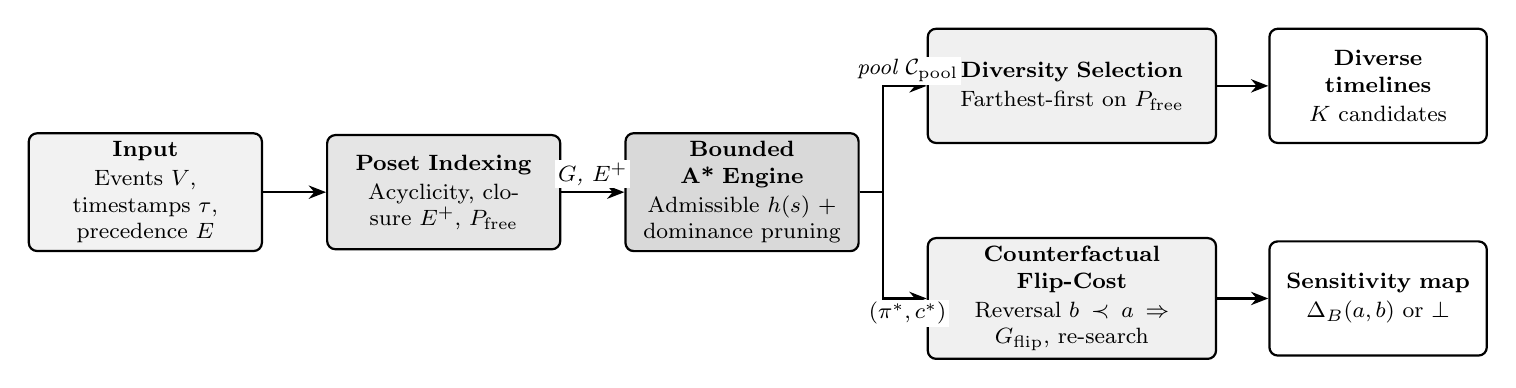
\begin{tikzpicture}[
  font=\footnotesize,
  box/.style={draw=black, rounded corners=3pt, thick, align=center, text width=2.75cm, minimum height=1.45cm, inner sep=3pt},
  wbox/.style={box, text width=3.45cm},
  obox/.style={box, text width=2.55cm},
  arr/.style={-{Stealth[length=2.2mm,width=1.7mm]}, thick},
  lab/.style={font=\footnotesize\itshape, align=center, inner sep=1pt, fill=white}
]
\node[box, fill=black!5] (in) at (1.45,0) {\textbf{Input}\\[1pt] Events $V$, timestamps $\tau$, precedence $E$};
\node[box, fill=black!10, right=0.8cm of in] (pi) {\textbf{Poset Indexing}\\[1pt] Acyclicity, closure $E^+$, $\Pfree$};
\node[box, fill=black!15, right=0.8cm of pi] (as) {\textbf{Bounded A* Engine}\\[1pt] Admissible $h(s)$ + dominance pruning};
\node[wbox, fill=black!6, right=0.85cm of as, yshift=1.35cm] (div) {\textbf{Diversity Selection}\\[1pt] Farthest-first on $\Pfree$};
\node[wbox, fill=black!6, right=0.85cm of as, yshift=-1.35cm] (cf) {\textbf{Counterfactual Flip-Cost}\\[1pt] Reversal $b\prec a\Rightarrow G_{\mathrm{flip}}$, re-search};
\node[obox, fill=white, right=0.65cm of div] (o1) {\textbf{Diverse timelines}\\[1pt] $K$ candidates};
\node[obox, fill=white, right=0.65cm of cf] (o2) {\textbf{Sensitivity map}\\[1pt] $\Delta_B(a,b)$ or $\bot$};

\draw[arr] (in) -- (pi);
\draw[arr] (pi) -- node[lab, above=1pt] {$G$, $E^+$} (as);
\draw[arr] (as.east) -- ++(0.3,0) |- node[lab, pos=0.78, above] {pool $\mathcal{C}_{\mathrm{pool}}$} (div.west);
\draw[arr] (as.east) -- ++(0.3,0) |- node[lab, pos=0.78, below] {$(\pi^*,c^*)$} (cf.west);
\draw[arr] (div) -- (o1);
\draw[arr] (cf) -- (o2);
\end{tikzpicture}
\end{document}
